\documentclass[10pt]{article}
\usepackage[utf8x]{inputenc}
\usepackage{polski}

\usepackage{amsmath}
\usepackage{amsthm}
\usepackage{amssymb}

\usepackage{graphics}
\usepackage{pdfpages}
\DeclareGraphicsRule{.1}{mps}{*}{}
\usepackage{epstopdf}
\usepackage{wrapfig}

\usepackage{geometry}
\geometry{a4paper, margin=2cm}

\begin{document}
    
%NAGLOWEK

    \noindent
    \begin{minipage}{0.5\textwidth}
        \LARGE{\textsf{\textbf{Zadanie: PUD\\Pudełka}}}
    \end{minipage}
    \begin{minipage}{0.5\textwidth}
        \begin{flushright}
            
\includegraphics[height=1.5cm]{logo.png}
        \end{flushright}
    \end{minipage}
    
    \noindent\rule{\textwidth}{0.4pt}
    
    \noindent\textbf{Akademia Programowania PWSW, dzień ?, Dostępna pamięć: 128 MB.}
    \vspace{1em}
    
%TRESC
    
    \noindent
    W magazynie Bajtockiej Wytwórni Papieru znajduje się $n$ pudełek, każde posiadające unikalny identyfikator (od 1 do $n$). Aby zaoszczędzić powierzchnię magazynu niektóre pudła wsadzono w inne (większe). Dlatego kiedy pracownicy potrzebują skompletować zamówienie muszą pamiętać, aby wyciągnąć nadmiarowe pudła, które nie zostały zamówione, a znajdują się we wnętrzu.

    Napisz program, który dla danego zamówienia, pomoże pracownikom określić, ile nadmiarowych pudeł znajduje się we wnętrzu zamówionego zestawu.
    
%WEJSCIE

    \section*{Wejście}
    
    W pierwszym wierszu standardowego wejścia znajduje się jedna liczba całkowita $n$ $(1\leq n\leq 10^{5})$, oznaczająca liczbę pudełek w magazynie. W drugim wierszu znajduje się ciąg $n$ liczb całkowitych $p_{1}, p_{2}, \ldots, p_{n}$, gdzie $p_{i}$ oznacza, w którym pudełku zostało schowane pudło o identyfikatorze $i$. Jeżeli liczba ta wynosi 0, to pudełko nie zostało schowane we wnętrzu innego. W trzecim wierszu znajduje się liczba całkowita $q$ $(1\leq q\leq 10^{5})$, oznaczająca liczbę zamównień testowych jakie ma rozpatrzeć nowy system (ponieważ jest to tylko test, stan magazynu nie zmienia się pomiędzy zamówieniami). W kolejnych $q$ liniach podane są zamówienia w następującym formacie: $m$ $(1 \leq m \leq 20)$ - liczba zamówionych pudełek, oraz $m$ liczb będących identyfikatorami tych pudełek.

%WYJSCIE

    \section*{Wyjście}
    
    Na standardowe wyjście należy wypisać $q$ linii, w każdej jedną liczbę całkowitą, oznaczającą liczbę nadmiarowych pudełek w $i$-tym zamówieniu.

%PRZYKLAD

    \section*{Przykład}
    
    \noindent
    \begin{minipage}[t]{0.5\textwidth}
        Dla danych wejściowych:\vspace{1ex}\\
        \texttt{5\\0 1 1 2 2\\5\\1 1\\2 4 5\\2 3 4\\3 2 3 4\\1 2}
    \end{minipage}
    \begin{minipage}[t]{0.5\textwidth}
        poprawnym wynikiem jest:\vspace{1ex}\\
        \texttt{4\\0\\0\\1\\2}       
    \end{minipage}
    
    
    \begin{wrapfigure}{r}{0.2\textwidth}
        \vspace{-3ex}
        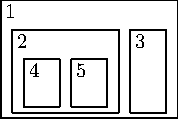
\includegraphics{pudrys-1.pdf}
    \end{wrapfigure}
    \vspace{2ex}
    \noindent\textbf{Wyjaśnienie przykładu:} Pierwsze zamówienie: W pierwszym pudełku znajdują się wszystkie pozostałe pudełka. Drugie i trzecie zamówienie: Pudełka 3, 4 i 5 nie zawierają żadnego pudełka we wnętrzu. Czwarte zamówienie: Nadmiarowe jest pudełko numer 5, które nie było zamówione. Piąte zamówienie: W pudełku numer dwa znajdują się dwa pudełka (3 i 4), których nie zamówiono.
    
%OCENIANIE

    \section*{Ocenianie}
        
    Zestaw testów dzieli się na następujące podzadania. Testy do każdego podzadania składają się z jednej lub większej liczby osobnych grup testów.
    
    \begin{center}
        \begin{tabular}{ |c|p{9cm}|c| }
            \hline
            \textbf{Podzadanie} & \textbf{Warunki} & \textbf{Liczba punktów}\\
            \hline
            1 & $1 \leq n, q \leq 1000$ & 30\\
            \hline
            2 & każde pudło jest wsadzone w co najwyżej jedno inne & 20\\
            \hline
            3 & brak dodatkowych ograniczeń & 50\\
            \hline
        \end{tabular}
    \end{center}

\end{document}
